\begin{landscape}

\subsection{Plan de la primera iteración}

\begin{figure}[H]
\centering
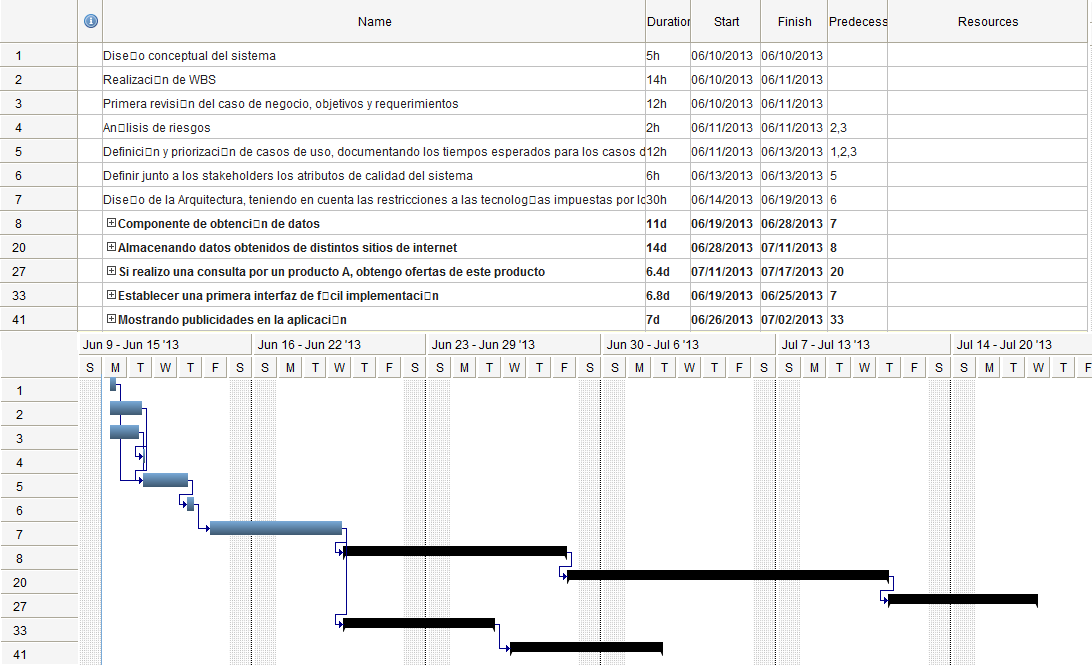
\includegraphics[scale=\escaladefault]{graficos/gantt/gantt.png}
\caption{El Gantt con las CU Comprimidas para una visualizacion completa}
\end{figure}

\begin{figure}[H]
\centering
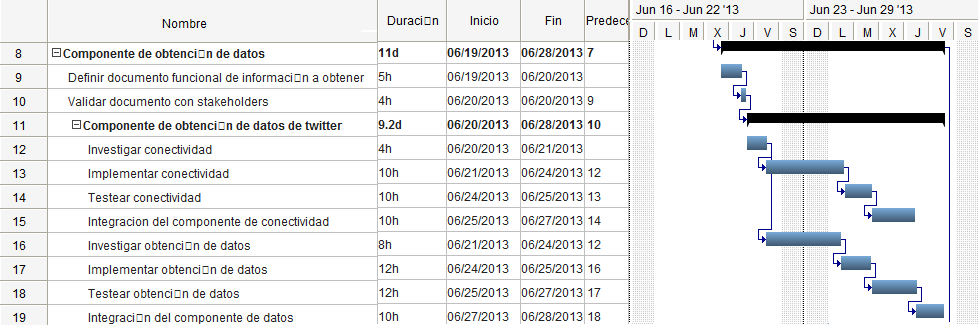
\includegraphics[scale=\escaladefault]{graficos/gantt/subgantt1.png}
\caption{Zoom sobre la CU de obtencion de datos}
\end{figure}

\begin{figure}[H]
\centering
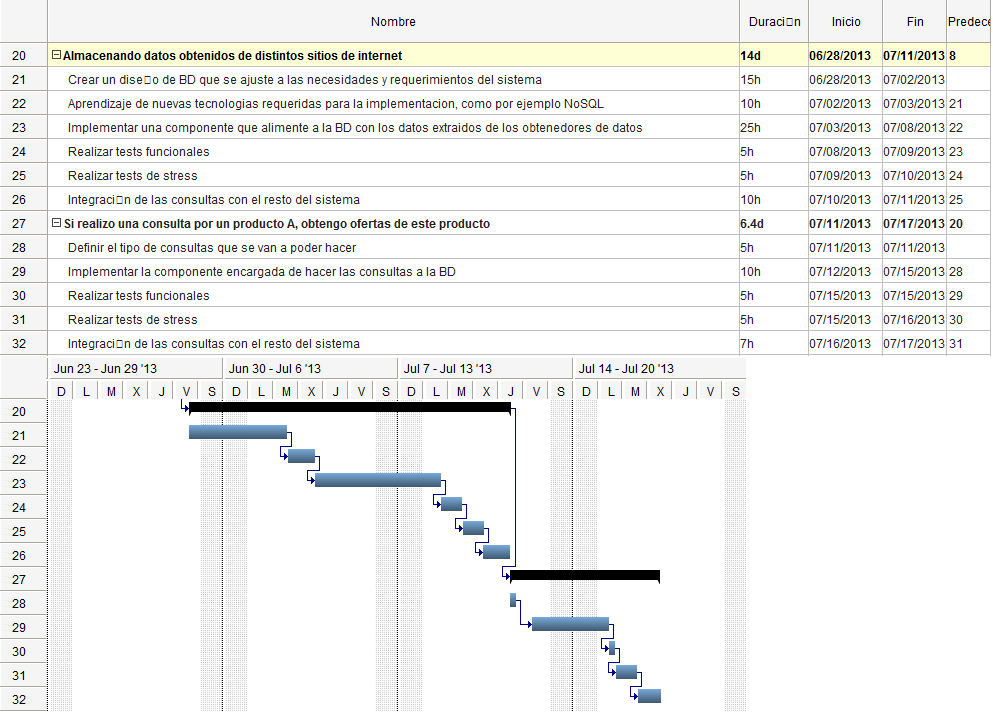
\includegraphics[scale=\escaladefault]{graficos/gantt/subgantt2.png}
\caption{}
\end{figure}

\begin{figure}[H]
\centering
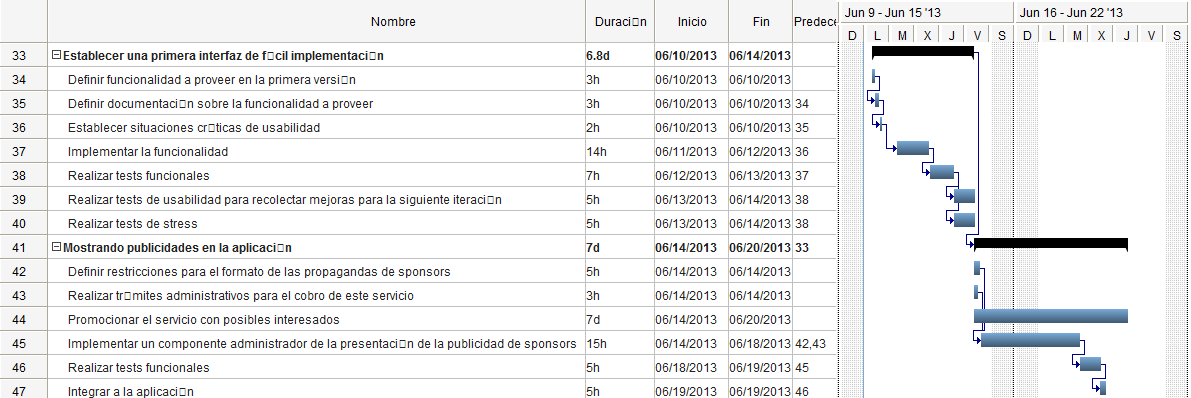
\includegraphics[scale=\escaladefault]{graficos/gantt/subgantt3.png}
\caption{}
\end{figure}

\end{landscape}